\chapter{Results of experiments with \carrp}
\label{app:cap}
\textit{In this appendix results values of experiments with \carrp{} are presented.}
\vfill
\newpage

Column labels:
\begin{itemize}
\item \texttt{Sequential}: Experiment using one core.
\item \texttt{No Communication}: Experiment using 40 cores without communication.
\item \texttt{St\_S / K \% com. OP}: Experiment with $K$\% of communicating solvers ($\tfrac{K}{2}$\% of sender solvers, and $\tfrac{K}{2}$\% of receiver solvers) using the communication strategy $S$ and the communication operator $OP$, and $100-K$\% of non-communicating solvers.
\begin{itemize}
\item Communication strategy:
	\begin{itemize}
	\item $S = a$: communication performed while applying the acceptance criteria 
	\item $S = b$: communication performed while performing a {\it reset} (each $k$ iterations)
	\item $S = c$: communication performed while performing a {\it reset} (each iteration)
	\end{itemize}
\item Communication operator:
	\begin{itemize}
	\item $OP = $ \texttt{1-1}: communication operator \texttt{one~to~one}
	\item $OP = $ \texttt{1-n}: communication operator \texttt{one~to~n}
	\end{itemize}
\end{itemize}
\item \texttt{Time}: Time in milliseconds. 
\item \texttt{Iter.}: Number of iterations.
\end{itemize}

Color caption:
\begin{itemize}
\item \gracias{Values in red color}: A receiver solver was the winner, finding the solution thanks to the received information.
\item \receiver{Values in dark red color}: A receiver solver was the winner, finding the solution without tacking into account the received information.
\item \sender{Values in blue color}: A sender solver was the winner.
\item \nocomm{Values in black color}: A non-communicating solver was the winner.
\end{itemize}

%\noindent\rule[2pt]{\textwidth}{0.8pt}

\clearpage
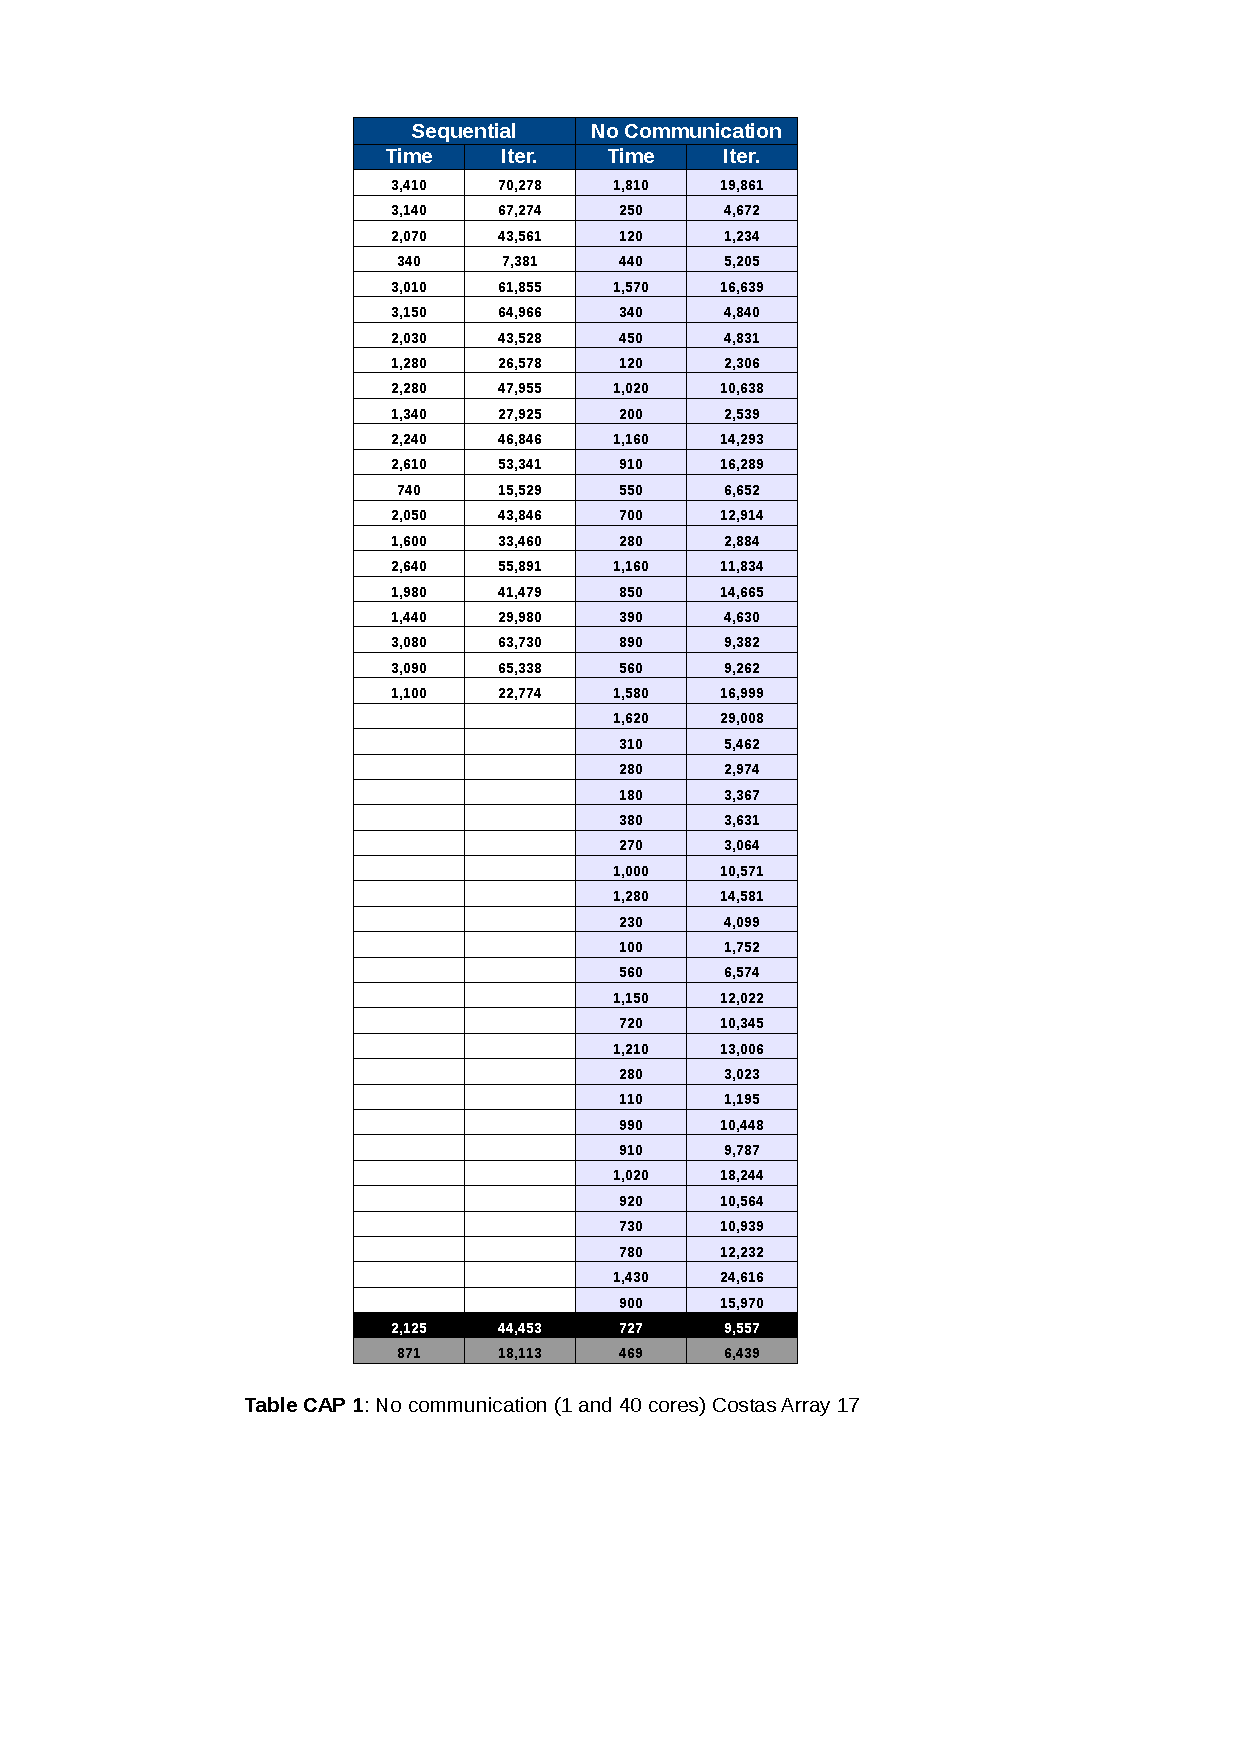
\includepdf[pages=-]{appres//res_costas.pdf}